%! TEX root = **/010-main.tex
% vim: spell spelllang=en:

\subsection{Support vector Machines}%
\label{sub:svm}

% discuss  choice  of  kernel  and  parameters used.  Did you run any method to speed the building of the model?
% Report number of supports of the selected machine and try to interpret why the kernel  selected  and
% parameters  selected  for  the  final  run  give  you  the best results for your dataset.
% Try also to inspect main supports of your machine.

\begin{figure}[H]
    \centering
    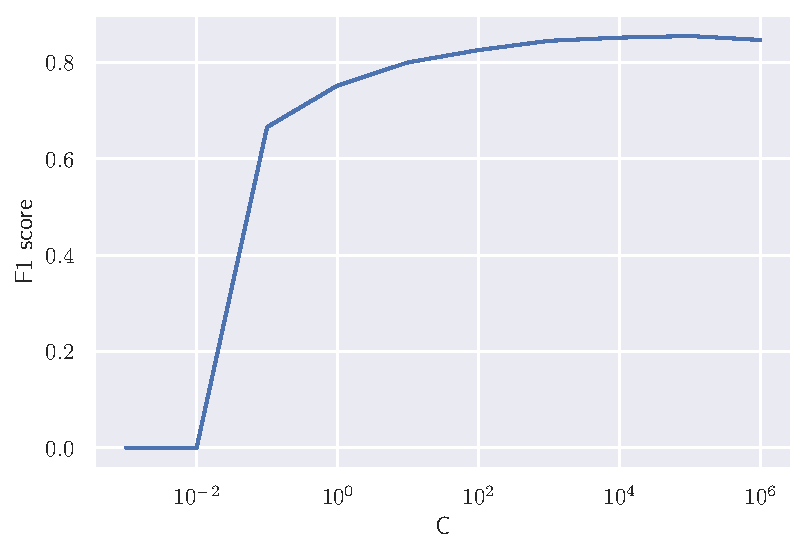
\includegraphics{svm_linear_C_cv}
    \caption{linear SVM C parameter search}%
    \label{fig:svm_linear_C_cv}
\end{figure}

\begin{figure}[H]
    \centering
    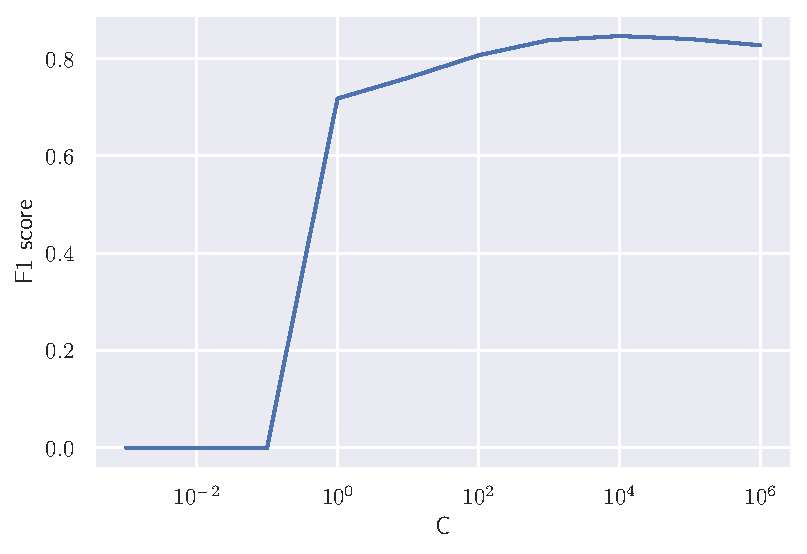
\includegraphics{svm_poly_C_cv}
    \caption{2nd degree polynomial SVM C parameter search}%
    \label{fig:svm_poly_C_cv}
\end{figure}

\begin{figure}[H]
    \centering
    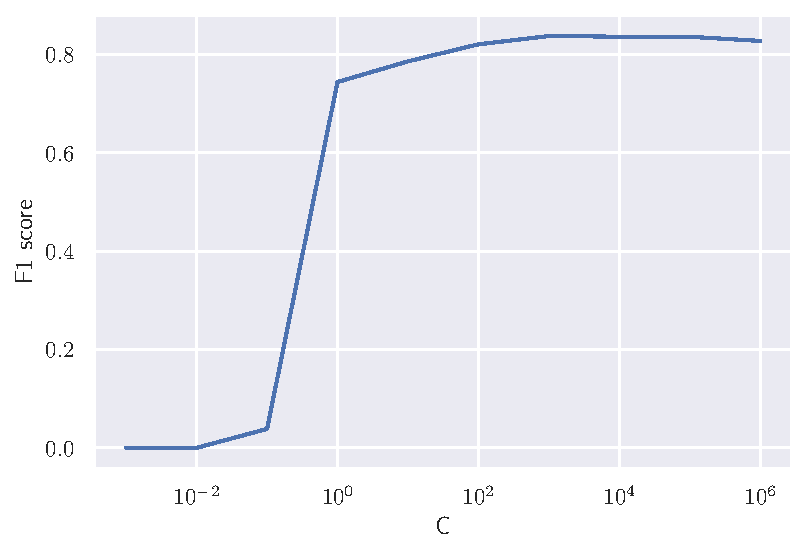
\includegraphics{svm_poly3_C_cv}
    \caption{3rd degree polynomial SVM C parameter search}%
    \label{fig:svm_poly3_C_cv}
\end{figure}

\begin{figure}[H]
    \centering
    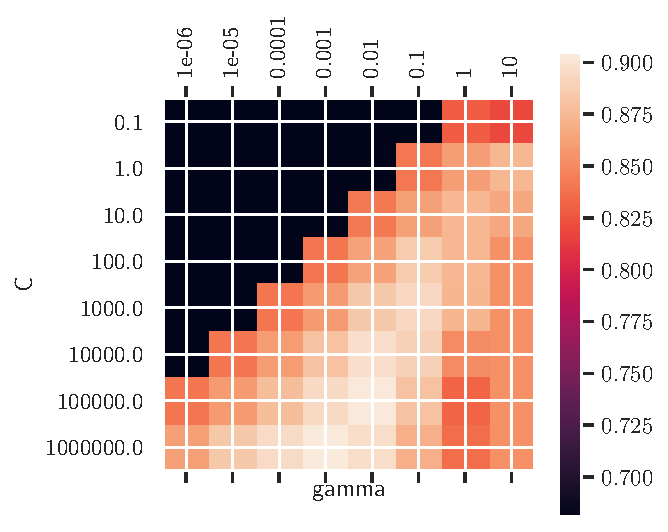
\includegraphics{svm_rbf_C_cv}
    \caption{RBF SVM C parameter search}%
    \label{fig:svm_rbf_C_cv}
\end{figure}
